\chapter{Escenario 3: modelo SQuaRE}
\sourcebadge{Actividad desarrollada literalmente desde el Documento Padre, escenario 3.}

La calidad interna observa código y arquitectura; la externa observa el comportamiento en pruebas; y la calidad en uso observa a usuarios que intentan alcanzar objetivos dentro de un contexto. Son perspectivas relacionadas, pero no intercambiables.

\begin{table}[H]\centering
\caption{Niveles de calidad aplicados a MediSalud}
\begin{tabularx}{\textwidth}{lX}\toprule
Nivel & Ejemplo\\\midrule
Interna & Complejidad y cobertura del módulo de facturación.\\
Externa & Prueba de carga del portal de citas con concurrencia controlada.\\
En uso & Tiempo real para registrar una nota durante consulta externa.\\\bottomrule
\end{tabularx}
\end{table}

\begin{figure}[H]\centering
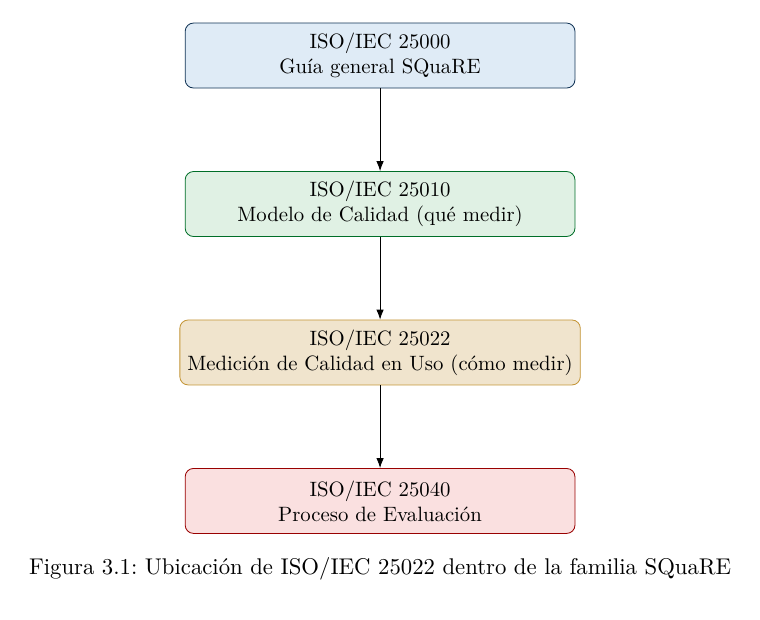
\includegraphics[width=0.62\textwidth]{figures/square.png}
\caption{Ubicación de ISO/IEC 25022 en la familia SQuaRE. Fuente: Documento Padre.}
\end{figure}

